\documentclass[12pt,a4paper]{article}
\usepackage[utf8]{inputenc}
\usepackage[english]{babel}
\usepackage[T1]{fontenc}
\usepackage{amsmath}
\usepackage{amsfonts}
\usepackage{amssymb}
\usepackage{graphicx}
\usepackage{siunitx}
\usepackage{float}
\usepackage[left=2cm,right=2cm,top=2cm,bottom=2cm]{geometry}
\author{Gerald}

\begin{document}
\sisetup{separate-uncertainty = true}
	\setlength{\parindent}{0pt} 
	\begin{center}
		{\LARGE Experiment protocol}\\
		\begin{large}
			for the solid state lab course\\[0.4cm]
			at RWTH Aachen\\
			II. Physikalisches Institut A\\[5.5cm]
			\Large\textbf{\textsl{Quantum Transport}}\\[5.5cm]
			\normalsize\textit{authored\\by}\\[0.4cm]
			\large{Moritz Berger (355244)\\Gerald Kolter (355005)}\\[2cm]
			\large \textbf{Summer term 2019}
		\end{large}
	\end{center}
	\newpage
	
	\tableofcontents
	\newpage

\section{Introduction}
At the interfaces between different materials the fermi levels align. Therefor the conduction and valence band bend. One can use this effect to create a two dimensional electron gas ("2DEG"). This is done by building a sample of thin layers of different materials. If done correctly, the conduction band bends underneath the Fermi level in one of the layer and is above it in every other layer. \\
With this structure one builds a hall probe, meaning a rectangular sample through which a current flows from side to side. The resistivity of the sample is measured parallel and perpendicular to this current. A variable magnetic field is applied perpendicular to the 2DEG. \\
At low temperatures the density of states in the 2DEG at zero magnetic field is a simple step function. With applying a magnetic field Landau levels are formed meaning the density of states becomes a function with single peaks, whose height, width and distance to each other depend on the magnetic field. As the Fermi energy stays the same, the density of states at the Fermi energy oscillates with the magnetic field. And as the resistivity depends mainly on the density of states at the Fermi energy the resistivity parallel to the magnetic field oscillates as well. These oscillations are called "Shubnikov-de Haas oscillations". \\
The resistivity perpendicular to the magnetic field depends linearly on the magnetic field and builds Hall plateaus.


\section{Goal of the Experiment}
The goal of the experiment is to determine different properties of the 2DEG: The charge carrier concentration $n_s$, the effective electron mass $m^*$, the quantum relaxation time $\tau _q$, the transport relaxation time $\tau _{tr}$ and the effective electrons' g-factor.


\section{Setup}
The 2DEG is build between a layer of GaAs and a layer of Al$_{x}$Ga$_{1-x}$As. For applying a magnetic field an electromagnet build from a superconductor is used. For the cooling a custom build cryostat is used. It consists out of an inner liquid helium (LHe) bath in which the sample is sunk. The LHe is sunk in an outer liquid nitrogen (LN) bath. Between these two an inner vacuum insulation and around the LN an outer vacuum insulation is formed for reducing heat conductance. \\
With this setup one can cool down the sample to \SI{4.2}{K}. To reach lower temperatures one pumps the gaseous helium out of the inner tube. With this one reaches the triple point of helium at around \SI{2.2}{K}.


\section{Measurement}
The magnetic field is sweeped from \SI{-5.4}{T} to \SI{5.4}{T}. Meanwhile the resistivity parallel and perpendicular to the current is measured. This is done at without pumping, meaning at about \SI{4.2}{K}, with a fractional pumping power, meaning at about \SI{3.5}{K}, and with maximal pumping power, meaning at about \SI{2.2}{K}.

\subsection{Data}

\begin{figure} [H]
\centering
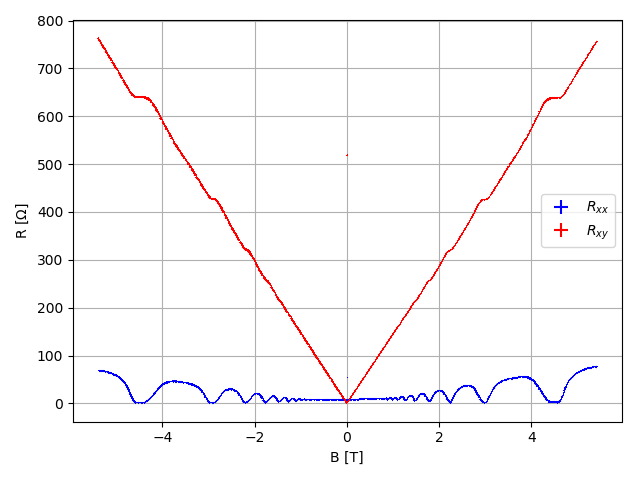
\includegraphics[scale=0.8]{Bilder/Elektron_g/4_2/Rohdaten.PNG}
\caption{Measured resistivities $R_{xx}$ and $R_{xy}$ in dependence of the magnetic field at \SI{4.2}{K}.}
\label{fig:raw_data}
\end{figure}

Fig. \ref{fig:raw_data} shows the measured raw data for the resistivities $R_{xx}$ and $R_{xy}$ in dependence of the magnetic field exemplary at \SI{4.2}{K}. The measurements at \SI{3.5}{K} and \SI{2.2}{K} yield similar results.



\section{Charge carrier concentration}
\subsection{Data analysis}


\subsection{Results}


\section{Effective electron mass}
\subsection{Data analysis}


\subsection{Results}



\section{Quantum relaxation time}
\subsection{Data analysis}


\subsection{Results}



\section{Transport relaxation time}
\subsection{Data analysis}

\subsection{Results}



\section{Electron effective g-faktor}
\subsection{Data analysis}

\subsection{Results}



\section{Conclusion}





%\begin{table} [H]
%\centering
%\begin{tabular}{|c|c|c|c|}
%\hline 
%$T_{room}$ [K] & $T_{LN_2}$ [K] & $R_{RT}$ [k$\Omega$] & $R_{LN_2}$ [k$\Omega$] \\ 
%\hline 
%294.65 $\pm$ $\frac{1}{\sqrt{12}}$ & 77 $\pm$ $\frac{1}{\sqrt{12}}$ & 107.9 $\pm$ $\frac{1}{\sqrt{12}}$ & 20.3 $\pm$ $\frac{1}{\sqrt{12}}$ \\ 
%\hline 
%\end{tabular} 
%\caption{Measured values for the resistance at room temperature and the temperature of liquid nitrogen.}
%\label{tab:Temp_Calib_data}
%\end{table}

%\begin{figure} [H]
%\centering
%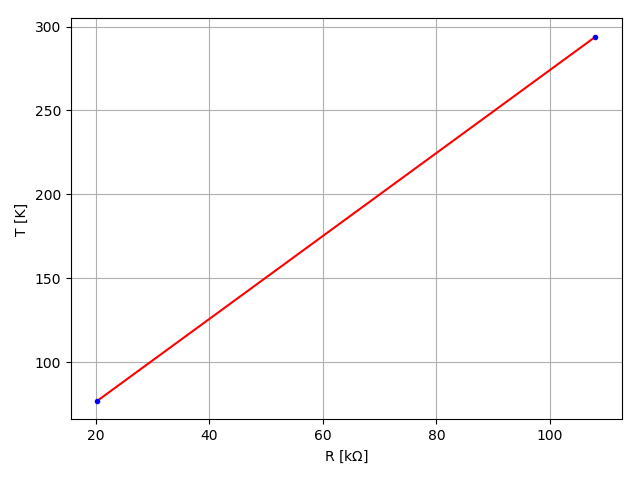
\includegraphics[scale=0.8]{Bilder/Temp_kalibration.PNG}
%\caption{Temperature calibration for the Pt-100 resistor.}
%\label{fig:Temp_kalibration}
%\end{figure}






\end{document}